% META: DONE.1

\section{Контур инференса и постобработка}

\subsection{Общая схема инференса}
Процесс инференса для пользовательской модели (STEP-файл) включает следующие шаги:

\begin{enumerate}
    \item \textbf{Триангуляция}: STEP-файл преобразуется в STL с адаптивным подбором параметра deflection (бинарный поиск), чтобы число треугольников не превышало 1500.
    \item \textbf{Нормализация и приведение рёбер}: STL переводится в OBJ, центрируется, масштабируется, и число рёбер доводится до 2250.
    \item \textbf{Запуск нейросети}: в зависимости от режима (автоматический или ручной) вызываются классификаторы и/или сегментаторы.
    \item \textbf{Постобработка}: из coloured OBJ извлекаются рёбра с меткой 1, формируется STL-файл выделенной геометрии.
    \item \textbf{Передача в КОМПАС-3D}: результаты (meta.json и test\_0.stl) передаются в CAD-среду для верификации и упрощения модели.
\end{enumerate}

\subsection{Режимы работы инференса}
Модуль поддерживает два режима, задаваемые параметром \texttt{--task}:

\begin{itemize}
    \item \textbf{Автоматический режим} (\texttt{--task auto}): последовательно вызываются классификаторы для всех доступных операций (исключая указанные в \texttt{--exclude}). Выбирается операция с наибольшей вероятностью, затем для неё запускается сегментация. Результат - файл \texttt{test\_0.stl} с геометрией, предположительно соответствующей этой операции, а также файл meta.json, в котором указано название выбранной операции и её вероятность.
    \item \textbf{Ручной режим} (\texttt{--task segmentation --operation <op>}): пользователь явно задаёт тип операции и параметры постобработки. Выполняется только сегментация или только классификация для указанной операции.
\end{itemize}

\subsection{Постобработка результатов сегментации}
Сеть возвращает раскрашенный OBJ-файл, где каждому ребру приписана метка 0 (фон) или 1 (операция). Для преобразования в STL выделенной геометрии применяются следующие алгоритмы:

\begin{enumerate}
    \item \textbf{Фильтрация по площади}: реализованная не как простое отсечение фиксированного процента крупнейших треугольников, а с применением статистического критерия на основе t-распределения Стьюдента. Для каждого набора треугольников, отнесённых сетью к операции, вычисляются среднее арифметическое и стандартное отклонение их площадей, а затем определяется верхняя граница доверительного интервала. Такой подход адаптивно работает с разными масштабами моделей и типами операций, в отличие от фиксированного порога по площади или процентиля, и помогает убрать выбросы - одиночные треугольники, ошибочно отнесённые к операции.
    \item \textbf{Кластеризация}: из всех треугольников, оставшихся после фильтрации, выделяется наибольший связный компонент (по рёберной смежности). Это позволяет отсеять разрозненные шумовые области (например, единичные ложные треугольники) и, что важно, разделить комплексные операции, состоящие из нескольких изолированных зон (например, множество отдельных вырезаний), на атомарные компоненты.
    \item \textbf{Преобразование рёбер в треугольники}: треугольник считается принадлежащим операции, если хотя бы два его ребра имеют метку 1 (экспериментально подобранный порог). Результирующая геометрия сохраняется в \texttt{test\_0.stl}.
\end{enumerate}

Дополнительно создаётся файл \texttt{meta.json}, содержащий для автоматического режима имя выбранной операции и её вероятность, или результаты классификации в общем случае.

\subsection{Схема работы}
Схема работы инференса представлена на рисунке ~\ref{fig:inference-pipeline}. Более подробная информация о работе инференса представлена в Приложении В.

\begin{figure}[h]
    \centering
    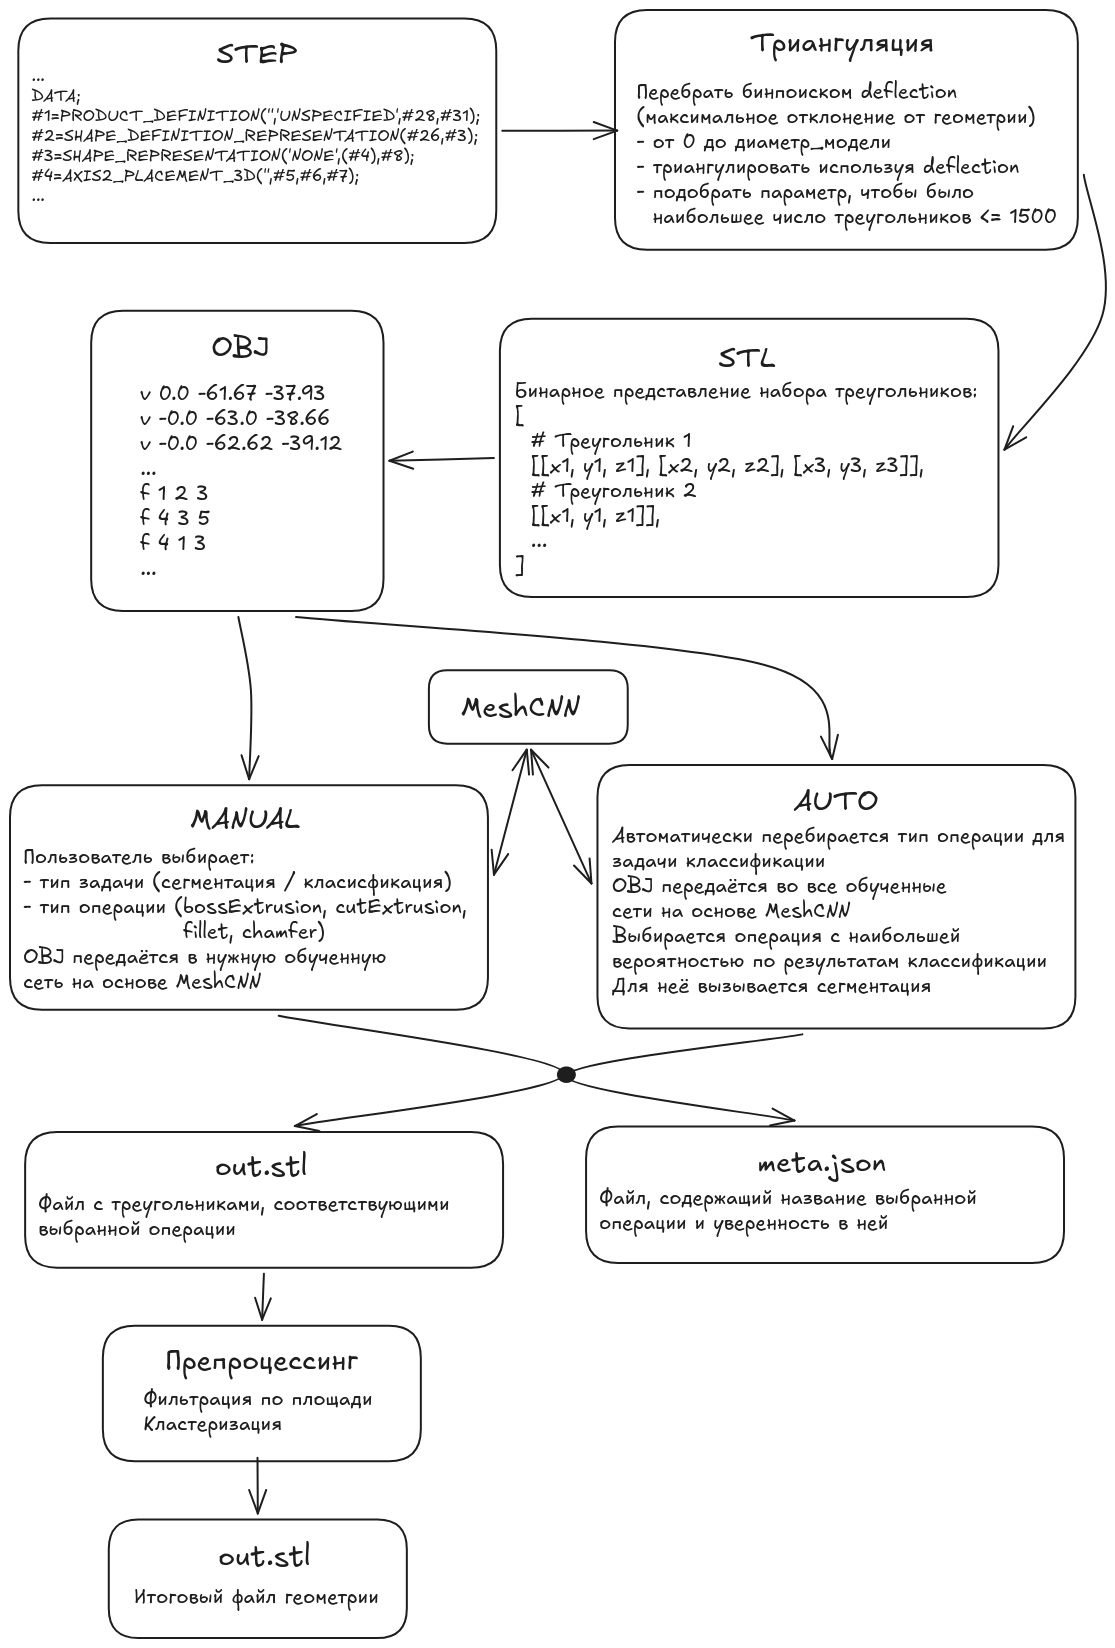
\includegraphics[width=0.7\linewidth]{figures/inference_pipeline.png}
    \caption{Схема работы исполняемого модуля}
    \label{fig:inference-pipeline}
\end{figure}

\subsection{Интеграция с КОМПАС-3D}
Разработанный модуль вызывается из внешнего скрипта или непосредственно из среды КОМПАС-3D через API. После получения \texttt{test\_0.stl} CAD-ядро выполняет следующие действия:
\begin{enumerate}
    \item Загружает выделенную геометрию и исходную модель (STEP).
    \item Детерминированно вычисляет параметры операции (например, для выдавливания - направление и глубину, для скругления - радиус).
    \item Пытается «отменить» операцию, т.е. получить модель до её применения.
    \item Если упрощение успешно, новая модель передаётся на следующий шаг итерации; если нет - гипотеза отвергается и выбирается следующая операция.
\end{enumerate}
Такой итеративный процесс позволяет постепенно восстановить дерево построения.

